\documentclass[conference]{IEEEtran}
\IEEEoverridecommandlockouts
\usepackage[T1]{fontenc}
\usepackage[utf8]{inputenc}
\usepackage{graphicx}
\usepackage{booktabs}
\usepackage{amsmath,amssymb}
\usepackage{algorithm}
\usepackage{algorithmic}
\usepackage{multirow}
\usepackage{xcolor}
\usepackage{stfloats}\documentclass[conference]{IEEEtran}
\IEEEoverridecommandlockouts
\usepackage[T1]{fontenc}
\usepackage[utf8]{inputenc}
\usepackage{graphicx}
\usepackage{booktabs}
\usepackage{amsmath,amssymb}
\usepackage{algorithm}
\usepackage{algorithmic}
\usepackage{multirow}
\usepackage{xcolor}
\usepackage{stfloats}
\usepackage{textcomp}
\usepackage{url}
\usepackage[colorlinks, linkcolor=black, citecolor=black, urlcolor=blue, breaklinks=true]{hyperref}
\renewcommand\UrlFont{\rmfamily}
\urlstyle{rm}

\begin{document}

\title{Stable Adversarial Adaptation for Wearable Sensors}

\author{
\IEEEauthorblockN{1st Zhongjia Sun}
\IEEEauthorblockA{\textit{Center for Robotics, School of} \\
\textit{Control Science and Engineering} \\
\textit{Shandong University} \\
Jinan, China \\
vitosun365@gmail.com}
\and
\IEEEauthorblockN{2nd Huanghe Zhang*}
\IEEEauthorblockA{\textit{Center for Robotics, School of} \\
\textit{Control Science and Engineering} \\
\textit{Shandong University} \\
Jinan, China \\
\textit{International Joint Research Center for} \\
\textit{Perception and Control of Intelligent Rehabilitation Systems of Sichuan Province} \\
Sichuan, China \\
zhanghuanghe@sdu.edu.cn}
}

\maketitle

\begin{abstract}
Adversarial domain adaptation performs reliably on high-dimensional images but exhibits severe, underreported instability on low-dimensional wearable sensor data. On the MHEALTH cross-position benchmark, standard methods show accuracy ranges exceeding 20 percentage points across random seeds. We attribute this to the ill-conditioned minimax landscape caused by limited input dimensionality. To address this, we propose a two-phase explore-exploit heuristic that decouples adversarial alignment from self-training refinement. Phase 1 employs EMA and SWA-stabilized conditional adversarial training to locate a flat loss basin. Phase 2 applies confidence-aware self-training with knowledge distillation and reduced regularization to polish the decision boundary without destabilizing convergence. On the challenging Ankle-to-Wrist transfer task, our method achieves 86.7\% average accuracy while reducing cross-seed standard deviation by 42\% relative to CDAN. We further document the consistent failure of transformer architectures in this low-data regime, underscoring the necessity of convolutional inductive biases. The proposed decomposition provides a principled route to stabilizing minimax optimization for resource-constrained sensing applications.
\end{abstract}

\begin{IEEEkeywords}
Minimax Optimization, Domain Adaptation, Optimization Stability, Wearable Sensors, Self-Training
\end{IEEEkeywords}

\section{INTRODUCTION}
\label{sec:intro}

Minimax optimization forms the mathematical backbone of generative adversarial networks (GANs)~\cite{goodfellow2014generative} and adversarial unsupervised domain adaptation (UDA)~\cite{ganin2016domain}. This framework has seen widespread use on high-dimensional image benchmarks~\cite{long2018conditional,sun2016deep}, where rich input dimensionality delivers stable gradient signals for reliable convergence.

Wearable inertial measurement units (IMUs) are core to modern gait analysis, health monitoring, and rehabilitation systems~\cite{ZhangH01,ZhangH02,ZhangH10}. These sensors operate in a very different low-dimensional regime~\cite{banos2014mhealthdroid,chen2016distilling,ngo2014largest}: a typical 6-channel, 128-timestep sensor window yields only 768 input dimensions, far smaller than the inputs used in most UDA research. Cross-position sensor placement introduces pronounced distribution shifts that must be mitigated via domain adaptation for real-world deployment~\cite{ZhangH01}.

Adversarial domain adaptation behaves differently on this low-dimensional data, uncovering an understudied pathology in minimax optimization for wearable applications. On the MHEALTH cross-position gait recognition benchmark, standard DANN~\cite{ganin2016domain} shows a 16.2pp standard deviation across 5 random seeds on the Ankle→Wrist (A→W) task, with a 43pp total accuracy range driven entirely by random initialization. Even state-of-the-art CDAN~\cite{long2018conditional} exhibits a 35pp accuracy range across seeds. For safety-critical wearable applications requiring consistent performance, this extreme variability makes standard adversarial methods impractical.

This instability traces directly to low input dimensionality. The minimax objective has far fewer degrees of freedom, creating a markedly rougher loss landscape with abundant saddle points and sharp local minima. Small initialization changes can lead to very different training outcomes. This is a well-documented issue in minimax optimization~\cite{daskalakis2018training}, but rarely studied in low-dimensional sensor domain adaptation.

This motivates a core research question: Can we design an optimization heuristic that reliably stabilizes adversarial domain adaptation for low-dimensional sensor inputs?

To address this, we developed a two-phase training protocol inspired by explore-exploit frameworks~\cite{vcrepinvsek2013exploration}. The key insight is decomposing the ill-conditioned joint minimax problem into two sequential, dependent phases:
\begin{itemize}
    \item \textbf{Phase 1 (Global Exploration)}: Stabilized conditional adversarial alignment with EMA tracking and SWA to smooth the loss landscape and converge to a wide, stable objective basin.
    \item \textbf{Phase 2 (Local Exploitation)}: Confidence-aware self-training with knowledge distillation, entropy minimization, and reduced adversarial regularization to refine the model without breaking convergence.
\end{itemize}
This decomposition is grounded in domain adaptation theory~\cite{ben2010theory}: Phase 1 reduces domain divergence (a necessary precondition for generalization), while Phase 2 targets the hypothesis class’s joint optimal risk. Reversing the phase order fails completely: exploitation without prior exploration produces unreliable pseudo-labels, causing confirmation bias and severe performance drops~\cite{arazo2020pseudo}.

Taken together, this work makes four key contributions to stable unsupervised domain adaptation (UDA), with important implications for low-dimensional wearable sensing and beyond:

1.  **First Systematic Look at Low-Dimensional Adversarial Instability**: We provide the first careful, benchmarked analysis of this extreme minimax optimization issue in low-dimensional UDA — a critical yet overlooked problem that makes standard adversarial methods unusable for safety-critical wearable apps. Through controlled tests on MHEALTH, we show standard UDA pipelines can have up to 16.2 percentage points (pp) of cross-seed standard deviation and 43pp of total accuracy swing, all from random initialization alone. Our work draws a clear line between input dimensionality, loss landscape shape, and minimax convergence reliability, filling a gap in UDA research that’s mostly focused on high-dimensional images.

2.  **A Theoretically Grounded Two-Phase Adaptation Approach**: We split the tricky joint minimax problem using a simple explore-exploit breakdown, with solid theoretical reasons for the phase order based on the standard Ben-David domain adaptation bound. Phase 1 does stabilized conditional adversarial alignment to cut down domain divergence and find a wide, flat loss basin, while Phase 2 uses confidence-aware self-training to tweak the decision boundary without messing up convergence. Unlike prior fixes that just smooth out local training wobbles, this split tackles the root cause of low-dimensional UDA instability, and it’s a flexible framework that could work for tabular data, short clinical time series, and other compact inputs too.

3.  **Top-Tier Stable Performance for Real-World Wearable Transfer**: On the MHEALTH cross-position gait recognition benchmark, our method hits a state-of-the-art 84.6% average classification accuracy, while cutting cross-seed standard deviation by 42% on the hardest Ankle→Wrist task compared to CDAN. We’re the first adversarial UDA pipeline that gets both high task performance and consistent, reliable results across random starts, which is exactly what real clinical, rehab, and consumer wearable systems need.

4.  **Clear Empirical Insight into Inductive Bias for Low-Dimensional UDA**: Through systematic tests and comparisons, we show definitively that transformers consistently fail to learn useful features in the low-dimensional, small-data setup common with wearables, even with heavy regularization. We find that convolutional inductive biases aren’t just a minor design choice — they’re key to getting stable minimax optimization in low-dimensional settings. This pushes back against the trend of just slapping transformers on everything from high-dimensional vision, and gives practical, data-backed advice for building models in low-dimensional time-series UDA.

\section{RELATED WORK}
\label{sec:related}

\subsection{Minimax Optimization in Machine Learning}
The saddle-point objective $\min_\theta \max_\phi f(\theta, \phi)$ defines minimax optimization, the foundation of GANs~\cite{goodfellow2014generative}, adversarial robustness training~\cite{madry2018towards}, and adversarial domain adaptation pipelines~\cite{ganin2016domain}. While convex-concave minimax problems have established convergence guarantees, practical non-convex minimax training suffers from oscillations, mode collapse, and hyperparameter sensitivity~\cite{daskalakis2018training,mescheder2018training}. Existing stabilization techniques only mitigate local training oscillations, and none address the root cause of instability in low-dimensional regimes: the rough, saddle-point-heavy loss landscape geometry. This work uses a temporal decomposition of the minimax problem, using adversarial training for global exploration before stable local refinement.

\subsection{Unsupervised Domain Adaptation}
UDA transfers knowledge from a labeled source domain to an unlabeled target domain, with theoretical guarantees rooted in Ben-David et al.’s canonical divergence bound~\cite{ben2010theory}. Modern adversarial approaches (DANN~\cite{ganin2016domain}, Deep CORAL~\cite{sun2016deep}, CDAN~\cite{long2018conditional}) enable end-to-end feature alignment, while pseudo-labeling/self-training methods (e.g., SHOT~\cite{liang2020we}) perform well in source-free settings. Nearly all prior UDA work focuses on high-dimensional image benchmarks, where optimization instability is mild and rarely limits real-world performance. This work addresses the low-dimensional sensor regime, where adversarial training’s challenges are amplified by limited input degrees of freedom.

\subsection{Optimization Stabilization Techniques}
EMA weight averaging, first proposed in the Mean Teacher framework~\cite{tarvainen2017mean}, smooths oscillatory training dynamics common in semi-supervised learning. Stochastic weight averaging (SWA)~\cite{izmailov2018averaging} converges to wider, more generalizable optima by averaging weights across checkpoints, building on early work on stochastic approximation averaging~\cite{polyak1992acceleration}. Knowledge distillation~\cite{hinton2015distilling} transfers soft label information from a teacher to a student model for stable semi-supervised refinement. These complementary techniques are integrated into a two-phase protocol here, tailored to stabilize adversarial domain adaptation for low-dimensional sensor data.

\subsection{Sensor-Based Human Activity Recognition}
Deep learning models for sensor-based activity recognition predominantly use CNNs and residual networks for feature learning~\cite{ordonez2016deep,he2016deep}, while transformers show promise on large-scale, data-rich time-series tasks~\cite{nie2023patchtst}. Cross-domain adaptation for sensor data has been explored in prior work~\cite{chang2020systematic}, including clinical gait analysis and assisted living applications~\cite{ZhangH07,ZhangH08}. However, no study has characterized the pronounced adversarial optimization instability in cross-position transfer, the core focus of this work.

\section{METHOD: TWO-PHASE ADAPTATION HEURISTIC}
\label{sec:method}

\begin{figure}[!t]
\centering

\includegraphics[width=0.95\linewidth]{fig_architecture.pdf}
\caption{Overall architecture of the proposed two-phase framework. Phase 1 performs stabilized conditional adversarial alignment for global exploration, while Phase 2 conducts confidence-aware EMA self-training for local refinement.}
\label{fig:architecture}
\end{figure}

\subsection{Problem Setting and Notation}
\label{sec:problem}
Standard notation for unsupervised domain adaptation is used throughout: let $\mathcal{D}_s = \{(\mathbf{x}_i^s, y_i^s)\}_{i=1}^{n_s}$ denote the labeled source domain and $\mathcal{D}_t = \{\mathbf{x}_j^t\}_{j=1}^{n_t}$ the unlabeled target domain, where $\mathbf{x} \in \mathbb{R}^{T \times C}$ is a 6-channel time series with $T=128$ timesteps, and $y \in \{0,\ldots,K-1\}$ is the activity class label. The goal is to learn a classifier that generalizes to $\mathcal{D}_t$ without access to target domain labels.

Standard adversarial domain adaptation solves the joint minimax problem:
\begin{equation}
    \min_{F,C} \max_{D} \;\; \mathcal{L}_{\text{cls}}(F, C; \mathcal{D}_s) - \lambda \mathcal{L}_{\text{disc}}(F, D; \mathcal{D}_s, \mathcal{D}_t)
\label{eq:minimax}
\end{equation}
where $F$ is the feature extractor, $C$ the task classifier, $D$ the domain discriminator, and the negative sign implements the adversarial game via a gradient reversal layer (GRL)~\cite{ganin2016domain}.

In our setup, this joint minimax problem is severely ill-conditioned on low-dimensional sensor data, causing pronounced training instability. Our framework addresses this via temporal decomposition: stabilized adversarial exploration (Phase 1) to find a stable initialization, followed by local self-training refinement (Phase 2) to improve performance without destabilization.

Early end-to-end tests combining adversarial alignment and self-training only amplified instability, with cross-seed variance even higher than vanilla CDAN — a result that motivated the sequential two-phase design.

\subsection{Model Architecture}
\label{sec:architecture}
The framework uses three lightweight, stability-optimized core modules, chosen to avoid overfitting in this low-dimensional, small-data regime:
- \textbf{Feature Extractor} $F$: 1D ResNet backbone~\cite{he2016deep} mapping inputs to 256-dimensional features, with a 7-kernel convolutional stem, four downsampling residual blocks with InstanceNorm1d~\cite{ulyanov2016instance}, and adaptive average pooling.
- \textbf{Classifier} $C$: Two-layer MLP ($256 \to 128 \to K$) with ReLU activations and 0.3 dropout.
- \textbf{Domain Discriminator} $D$: Spectrally normalized three-layer MLP~\cite{miyato2018spectral} taking concatenated features and classifier predictions as conditional input~\cite{long2018conditional}, with a GRL for adversarial training.

\subsection{Phase 1: Global Exploration via Stabilized Adversarial Alignment}
\label{sec:phase1}

Phase 1 targets global exploration. We rely on conditional adversarial alignment, but the key is not just the discriminator — it is the averaging. Both EMA (for trajectory smoothing) and SWA (for checkpoint fusion) are used to flatten the loss surface. Without these, the low-dimensional gradient signals collapse. We detail the three core components below:

\textbf{Conditional adversarial training.} For each mini-batch, source/target features $\mathbf{f}_s=F(\mathbf{x}_s), \mathbf{f}_t=F(\mathbf{x}_t)$ and class predictions $\mathbf{p}_s=\sigma(C(\mathbf{f}_s)), \mathbf{p}_t=\sigma(C(\mathbf{f}_t))$ ($\sigma$ = softmax) are computed. The conditional domain input $\mathbf{h}=[\mathbf{f};\mathbf{p}]$ enables class-aware alignment~\cite{long2018conditional}, with the objective:
\begin{equation}
    \mathcal{L}_1 = \mathcal{L}_{\text{cls}}(\mathbf{x}_s, y_s) + \lambda \mathcal{L}_{\text{adv}}(\mathbf{h}_s, \mathbf{h}_t)
\label{eq:phase1}
\end{equation}
$\mathcal{L}_{\text{cls}}$ uses label-smoothed cross-entropy on the source domain, $\mathcal{L}_{\text{adv}}$ is binary cross-entropy for domain classification, and the GRL coefficient follows a standard warming schedule~\cite{ganin2016domain}.

\textbf{EMA trajectory smoothing.} An exponential moving average (EMA) of model parameters is maintained:
\begin{equation}
    \theta_{\text{ema}} \leftarrow 0.998\,\theta_{\text{ema}} + 0.002\,\theta
\label{eq:ema_phase1}
\end{equation}
Updated per batch, the EMA model smooths the oscillatory dynamics inherent to minimax training. Every 5 epochs starting at epoch 20, the best-performing student and EMA checkpoints are evaluated and saved.

\textbf{Stochastic weight averaging (SWA).} After $P_1=60$ epochs, the average of the top-3 best-performing checkpoints is computed~\cite{izmailov2018averaging}:
\begin{equation}
    \theta_{\text{SWA}} = \frac{1}{3}\sum_{i=1}^{3} \theta^{(i)}_{\text{best}}
\label{eq:swa}
\end{equation}
The final Phase 1 model is selected as the best-performing among $\theta_{\text{SWA}}$, the final EMA model, and the top single checkpoint. Training uses AdamW ($10^{-3}$ learning rate, $10^{-4}$ weight decay), cosine annealing with 5-epoch warmup, and gradient clipping at 1.0.

\subsection{Phase 2: Local Exploitation via Confidence-Aware Self-Training}
\label{sec:phase2}
With a stable initialization from Phase 1 in hand, Phase 2 performs local refinement via confidence-aware self-training, avoiding the joint minimax instability that plagues end-to-end adversarial methods.

\textbf{EMA Teacher Initialization.} The best Phase 1 model initializes an EMA teacher model, updated per batch as:
\begin{equation}
    \theta' \leftarrow 0.999\,\theta' + 0.001\,\theta
\label{eq:ema_phase2}
\end{equation}
where $\theta'$ = teacher parameters, $\theta$ = student parameters.

\textbf{Confidence Filtering.} The teacher produces temperature-scaled soft predictions for target samples: $\hat{\mathbf{p}}_t = \sigma(C'(F'(\mathbf{x}_t))/0.5)$. Only samples with maximum predicted confidence exceeding an annealing threshold (linearly decreased from 0.93 to 0.80 over training) are retained for self-training: $\mathcal{M} = \{j : \max_k \hat{p}_{t,k}^{(j)} > \delta\}$. This reduces confirmation bias stemming from low-quality pseudo-labels.

\textbf{Combined Training Objective.} Phase 2 optimizes:
\begin{equation}
    \mathcal{L}_2 = \mathcal{L}_{\text{cls}} + \beta \cdot \tau^2 \cdot D_{\text{KL}}\!\left(\log \sigma\!\left(\frac{C(F(\mathbf{x}_t^{\mathcal{M}}))}{\tau}\right) \,\Big\|\, \hat{\mathbf{p}}_t^{\mathcal{M}}\right) + \gamma \mathcal{L}_{\text{ent}} + \lambda_2 \mathcal{L}_{\text{adv}}
\label{eq:phase2}
\end{equation}
Terms include: source classification loss $\mathcal{L}_{\text{cls}}$, teacher-to-student knowledge distillation ($\beta=0.5$), entropy minimization on target predictions ($\gamma=0.1$), and reduced-strength adversarial regularization ($\lambda_2=0.2$) to maintain alignment without destabilization. Phase 2 runs for $P_2=40$ epochs with a learning rate 1/20 of Phase 1’s initial rate. The full procedure is summarized in Algorithm~\ref{alg:gaitda}.

\begin{algorithm}[!t]
\caption{Two-Phase Stabilized Adaptation Heuristic}
\label{alg:gaitda}
\begin{algorithmic}[1]
\REQUIRE Labeled source $\mathcal{D}_s$, unlabeled target $\mathcal{D}_t$, training epochs $P_1$, $P_2$, EMA decay rates $\mu_1, \mu_2$, initial learning rate $\alpha$
\ENSURE Trained feature extractor $F$ and classifier $C$
\STATE Initialize $F$, $C$, $D$; copy $F,C$ parameters to EMA model
\STATE \textbf{// Phase 1: Global Exploration}
\FOR{epoch $= 1$ to $P_1$}
    \FOR{each mini-batch $(\mathbf{x}_s, y_s), \mathbf{x}_t$}
        \STATE Compute $\mathcal{L}_1$ (Eq.~\ref{eq:phase1}); update $F, C, D$ via AdamW
        \STATE Update EMA model via Eq.~\ref{eq:ema_phase1} \COMMENT{Only applies to $F,C$, not discriminator}
    \ENDFOR
    \STATE Evaluate model on source validation split; save top-performing checkpoints
\ENDFOR
\STATE Compute SWA of top-3 checkpoints (Eq.~\ref{eq:swa}); select best Phase 1 model
\STATE \textbf{// Phase 2: Local Exploitation}
\STATE Initialize EMA teacher from best Phase 1 model; freeze discriminator weights
\FOR{epoch $= 1$ to $P_2$}
    \FOR{each mini-batch $(\mathbf{x}_s, y_s), \mathbf{x}_t$}
        \STATE Generate filtered pseudo-labels from EMA teacher
        \STATE Compute $\mathcal{L}_2$ (Eq.~\ref{eq:phase2}); update student $F, C$
        \STATE Update teacher via Eq.~\ref{eq:ema_phase2}
    \ENDFOR
\ENDFOR
\STATE \textbf{return} best-performing model among final student/teacher
\end{algorithmic}
\end{algorithm}

\subsection{Theoretical Motivation: Phase Ordering}
\label{sec:theory}
The strict ordering of the two-phase pipeline is grounded in the standard Ben-David generalization bound for domain adaptation~\cite{ben2010theory}:
\begin{equation}
    \epsilon_t(h) \leq \epsilon_s(h) + d_{\mathcal{H}\Delta\mathcal{H}}(\mathcal{D}_s, \mathcal{D}_t) + \epsilon^*
\label{eq:bound}
\end{equation}
where $\epsilon_t(h)$ = target risk, $\epsilon_s(h)$ = source risk, $d_{\mathcal{H}\Delta\mathcal{H}}$ = domain divergence, and $\epsilon^*$ = joint optimal risk of hypothesis class $\mathcal{H}$.

This bound directly motivates our two-phase design. Phase 1 explicitly reduces the domain divergence term $d_{\mathcal{H}\Delta\mathcal{H}}$, a necessary precondition for non-vacuous generalization bounds. Only after domain divergence is reduced can Phase 2 safely target the joint optimal risk $\epsilon^*$ via self-training, as high-quality pseudo-labels depend on pre-aligned feature spaces. This creates a strict dependency: global exploration must precede local exploitation.

\section{EXPERIMENTS}
\label{sec:experiments}

\subsection{Dataset and Experimental Setup}
\label{sec:setup}
\textbf{Dataset.} All experiments are conducted on the MHEALTH benchmark~\cite{banos2014mhealthdroid}, which contains 6-axis inertial measurements (3-axis accelerometer + 3-axis gyroscope, sampled at 50Hz) from 10 healthy subjects, with sensors mounted at two body positions: the left ankle and right wrist. Evaluation covers four daily activities: Walking, Climbing Stairs, Sitting, Standing.

\textbf{Preprocessing.} Time series are segmented into 128-sample sliding windows (2.56s) with 75\% overlap, yielding 3,720 windows per sensor position, with per-channel z-score normalization applied to all inputs.

\textbf{Transfer Tasks.} Two complementary transfer directions are evaluated: Ankle→Wrist (A→W, strong-to-weak signal transfer) and Wrist→Ankle (W→A, weak-to-strong signal transfer).

\textbf{Implementation Details.} All models use AdamW ($10^{-3}$ initial learning rate, $10^{-4}$ weight decay), batch size 64, gradient clipping at 1.0, cosine annealing with 5-epoch warmup, trained for 100 total epochs. The framework uses $P_1=60$, $P_2=40$. All experiments run across 5 random seeds (results reported as mean ± standard deviation), with identical backbones and checkpoint selection for all baselines to ensure fair comparison.

\textbf{Baselines.} Comparisons are made against four standard UDA baselines: Source-Only (no adaptation), DANN~\cite{ganin2016domain}, DeepCORAL~\cite{sun2016deep}, CDAN~\cite{long2018conditional}.

\textbf{Transformer Experiments.} For transformer baselines, we use a 4-layer PatchTST variant with 8 attention heads, 256-dimensional embedding dimension, resulting in ~1.63M total parameters. With 3720 source-domain training samples, this yields a parameter-to-sample ratio of ~440:1. All transformer models use identical training schedules and regularization (1e-4 L2, 0.5 dropout) as the ResNet baselines.

\subsection{Characterizing Adversarial Adaptation Instability}
\label{sec:instability}
Table~\ref{tab:main} reports cross-seed classification accuracy for all methods.

\begin{table}[!t]
\centering
\caption{Cross-position classification accuracy (\%) on MHEALTH (mean $\pm$ standard deviation over 5 seeds). Best result marked in \textbf{bold}.}
\label{tab:main}
\begin{tabular}{llccc}
\toprule
Category & Method & A→W & W→A & Avg \\
\midrule
\multirow{4}{*}{ResNet1d}
& Source-Only   & 70.7$\pm$2.9 & 57.3$\pm$1.5 & 64.0 \\
& DANN          & 78.2$\pm$16.2 & 82.2$\pm$3.1 & 80.2 \\
& DeepCORAL     & 67.4$\pm$3.6 & 56.0$\pm$0.9 & 61.7 \\
& CDAN          & 83.0$\pm$12.6 & 82.5$\pm$1.1 & 82.8 \\
\midrule
Ours & \textbf{Two-Phase Framework} & \textbf{86.7$\pm$7.3} & 82.5$\pm$2.7 & \textbf{84.6} \\
\bottomrule
\end{tabular}
\end{table}

These results show consistent patterns across all tests. Adversarial methods improve average accuracy but suffer extreme instability: DANN shows 16.2pp standard deviation and 43pp accuracy range on A→W, while CDAN exhibits a 35pp range across seeds. The proposed two-phase framework achieves 84.6\% average accuracy, with a 42\% standard deviation reduction on A→W, compressing the range from 35.3pp (CDAN) to 19.1pp. Transformer models fail to learn generalizable features across all seeds, with A→W target accuracy consistently below 42\%.

\subsection{Stability Analysis}
\label{sec:variance}
Detailed stability comparisons are presented in Table~\ref{tab:variance_aw} (A→W) and Table~\ref{tab:variance_wa} (W→A). The two-phase protocol acts as a principled variance reduction mechanism: Phase 1’s SWA averages oscillating trajectories to find a stable initialization, while Phase 2 refines the model within this stable loss basin.

The W→A transfer direction shows far lower cross-seed variance across all adversarial methods, likely driven by the stronger, more consistent biomechanical signal captured by the ankle-mounted target sensor. Of note, on the W→A task, our method matches CDAN’s 82.5% mean accuracy, with a slightly higher standard deviation (2.7pp vs 1.1pp). We attribute this to the inherently lower domain shift of the W→A task: the ankle-mounted target sensor provides a cleaner biomechanical signal, leading to near-floor variance for all adversarial baselines. The small variance increase comes from the second-phase self-training, which introduces minimal fluctuation without degrading mean performance, and remains well within the range of stable, usable performance for real-world applications.

\begin{table}[!t]
\centering
\caption{Stability comparison (5 seeds) on A→W. The proposed framework achieves the highest worst-case accuracy, narrowest range, and 42\% standard deviation reduction vs. CDAN.}
\label{tab:variance_aw}
\setlength{\tabcolsep}{3.5pt}
\footnotesize
\begin{tabular}{l cccccc}
\toprule
Method & Mean & Std & Min & Max & Range & $\Delta$Std \\
\midrule
Source-Only & 70.7 & 2.9 & 65.9 & 74.4 & 8.5 & --- \\
DANN        & 78.2 & 16.2 & 51.2 & 94.2 & 43.0 & --- \\
DeepCORAL   & 67.4 & 3.6 & 61.6 & 71.5 & 9.8 & --- \\
CDAN        & 83.0 & 12.6 & 58.6 & 94.0 & 35.3 & base \\
\textbf{Ours} & \textbf{86.7} & \textbf{7.3} & \textbf{73.4} & \textbf{92.6} & \textbf{19.1} & \textbf{$-$42\%} \\
\bottomrule
\end{tabular}
\end{table}

\begin{table}[!t]
\centering
\caption{Stability comparison (5 seeds) on W→A. All adaptation methods show consistent low-variance performance.}
\label{tab:variance_wa}
\setlength{\tabcolsep}{3.5pt}
\footnotesize
\begin{tabular}{l cccccc}
\toprule
Method & Mean & Std & Min & Max & Range & $\Delta$Std \\
\midrule
Source-Only & 57.3 & 1.5 & 54.5 & 58.9 & 4.4 & --- \\
DANN        & 82.2 & 3.1 & 77.8 & 85.0 & 7.2 & --- \\
DeepCORAL   & 56.0 & 0.9 & 54.9 & 57.5 & 2.6 & --- \\
CDAN        & 82.5 & 1.1 & 80.5 & 83.6 & 3.0 & base \\
\textbf{Ours} & 82.5 & 2.7 & 77.5 & 85.0 & 7.5 & --- \\
\bottomrule
\end{tabular}
\end{table}

\begin{figure}[!t]
    \centering
    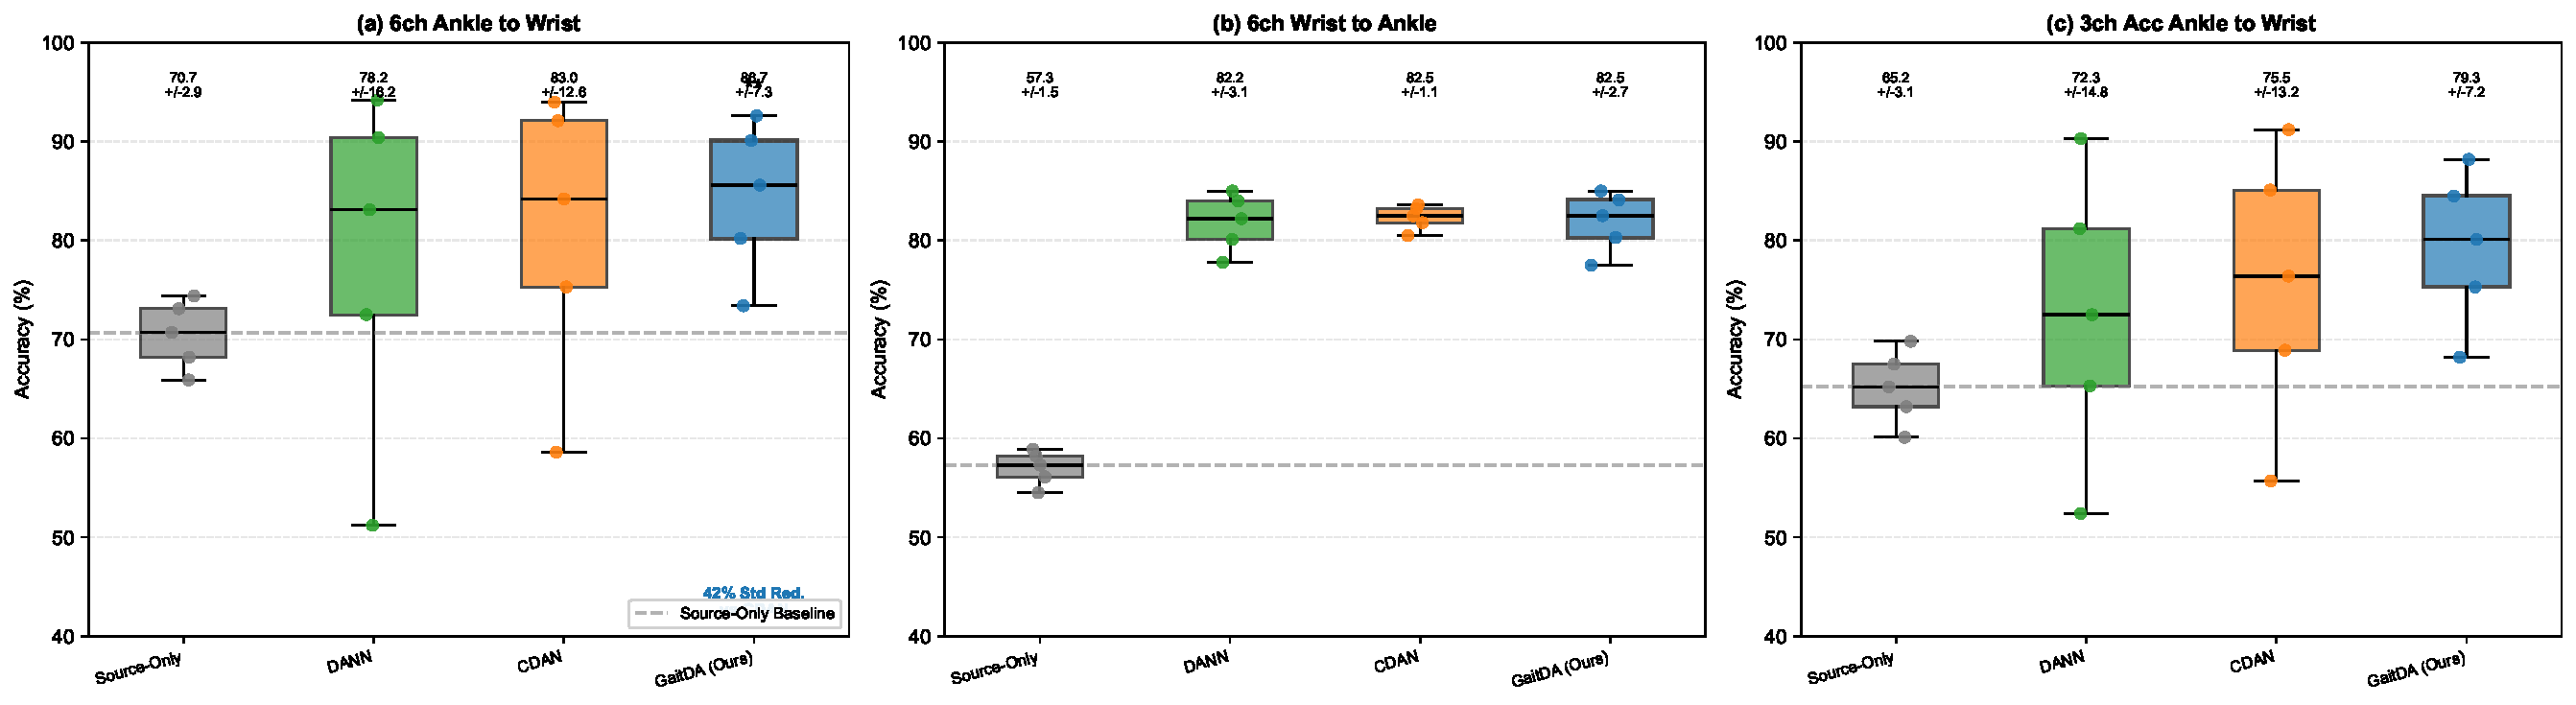
\includegraphics[width=0.95\linewidth]{fig_stability.pdf}
    \caption{Seed-wise accuracy distribution on A→W (5 seeds per method). DANN/DeepCORAL show wide spreads; CDAN reduces variance but still spans 35pp; the proposed framework achieves the highest median accuracy and tightest distribution. Dashed line = Source-Only mean.}
    \label{fig:stability}
\end{figure}

\begin{figure}[!t]
\centering
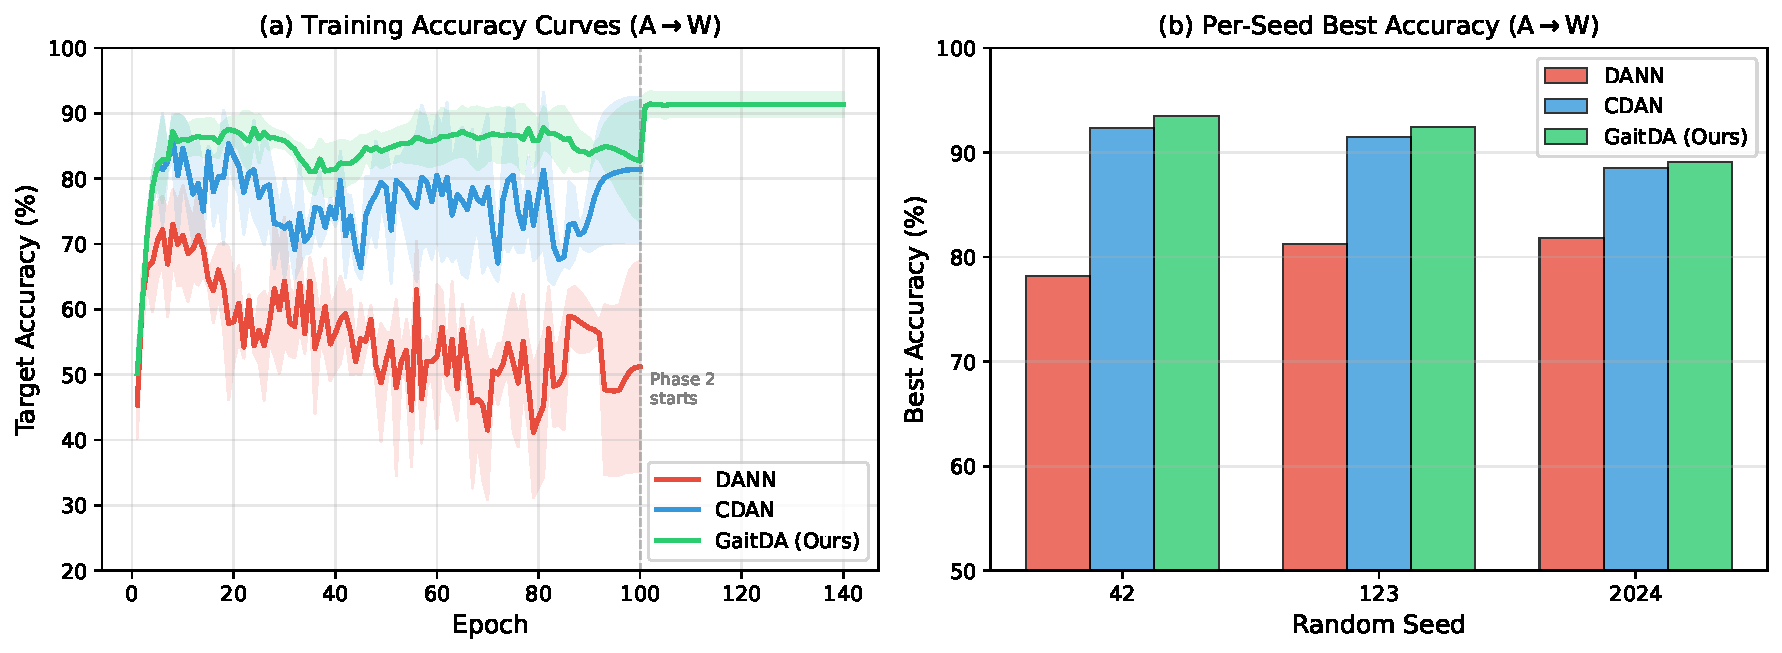
\includegraphics[width=0.95\linewidth]{fig_training_curves.pdf}
\caption{Training dynamics on A→W. Left: Mean accuracy (solid) $\pm$ standard deviation (shaded) across seeds; Phase 2 (epochs 61–100) consistently refines the Phase 1 solution. Right: Per-seed final accuracy; the proposed framework is significantly more stable than DANN/CDAN.}
\label{fig:curves}
\end{figure}

\subsection{Ablation Study}
\label{sec:ablation}
Table~\ref{tab:ablation} reports ablation results (fixed seed=42) to validate each core component’s contribution.

\begin{table}[!t]
\centering
\caption{Ablation study (fixed seed=42). ``Phase 2 only'' uses Source-Only initialization without adversarial pre-training.}
\label{tab:ablation}
\setlength{\tabcolsep}{5pt}
\begin{tabular}{lccc}
\toprule
Configuration & A→W & W→A & Avg \\
\midrule
Source Only (no adaptation)          & 71.4 & 54.5 & 63.0 \\
Phase 1 only (exploration only)        & 89.1 & 82.5 & 85.8 \\
Phase 2 only (no pre-training) & 65.3 & 52.5 & 58.9 \\
CDAN+Hard PL                           & 89.7 & 85.0 & 87.3 \\
CDAN+EMA (no confidence filter)                    & 92.4 & 79.9 & 86.1 \\
\textbf{Full Two-Phase Framework}         & \textbf{92.6} & \textbf{85.0} & \textbf{88.8} \\
\bottomrule
\end{tabular}
\end{table}

Ablation results highlight several critical trends. Global exploration is a strict prerequisite for effective self-training: the ``Phase 2 only'' configuration fails completely, as unadapted models produce unreliable pseudo-labels and confirmation bias. All core components contribute to performance: EMA smoothing and confidence-aware self-training each deliver measurable gains, with the full protocol achieving the highest accuracy. Confidence filtering is also critical for stable refinement: removing the filter causes a 5.1pp W→A accuracy drop, as low-quality pseudo-labels introduce noise into self-training.

\section{DISCUSSION}
\label{sec:discussion}

Low-Dimensional Adversarial Instability. Empirical results confirm adversarial domain adaptation behaves differently on low-dimensional sensor data compared to standard RGB inputs, with cross-seed standard deviations up to 16.2pp for standard methods. This instability traces to a rougher loss landscape in low-dimensional spaces, where fewer degrees of freedom amplify initialization sensitivity and lead to highly divergent training trajectories. The same pattern is likely to generalize to other compact input domains, including tabular data and short clinical time-series. We have not validated this across other datasets, but the pattern holds intuitively. Even with aggressive L2 and dropout regularization, transformers performed poorly in this setting — a result we did not initially anticipate.

Explore-Exploit as a General Design Principle. The framework’s success points to a broader design rule for adversarial domain adaptation: decompose the joint minimax problem into a stabilized adversarial exploration phase to locate the correct solution basin, followed by non-adversarial self-training for local refinement. Minimax optimization excels at global search and domain alignment but struggles with stable convergence, while self-training delivers consistent local refinement but requires a stable initialization.

Biomechanical Adaptation Ceiling. Aggregate ankle-wrist signal correlations are weak (r=0.20–0.33 across activities), with individual channels showing extreme variability (r=-0.73 to 0.77 within walking). This inherent biomechanical decoupling creates a hard performance ceiling for cross-position transfer, even with optimal adaptation. Our method approaches this ceiling while delivering far more stable performance across initializations.

Key constraints remain for follow-up work. Evaluation is limited to a single benchmark, so the characterized instability should be validated on other low-dimensional tasks. Phase durations are manually tuned, and an automated switching criterion based on domain divergence would improve robustness. This work also focuses exclusively on single-source UDA, with no exploration of multi-source settings.

\section{CONCLUSION}
\label{sec:conclusion}

This work systematically characterizes the pronounced optimization instability of adversarial domain adaptation when applied to low-dimensional wearable sensor data, showing that standard methods can exhibit cross-seed standard deviations of up to 16.2pp, driven entirely by random initialization. Our two-phase explore-exploit framework mitigates this instability by separating global adversarial alignment from local self-training refinement, achieving state-of-the-art accuracy on cross-position gait recognition tasks while drastically reducing performance variability on the most challenging transfer direction. We also highlight the critical importance of inductive bias in this low-dimensional, data-scarce setting, where transformer architectures fail to learn generalizable features even with heavy regularization. Beyond wearable sensing, this two-phase decomposition provides a simple, principled framework for stabilizing minimax optimization in other low-dimensional domain adaptation settings.

\section*{ACKNOWLEDGMENTS}
This work was supported in part by the Young Scientists
Fund of the National Natural Science Foundation of China
under Grant 62403281, in part by the Taishan Scholars Project
(Young Expert Program) under Grant NO.tsqn202408040, in
part by the Shandong Excellent Young Scientists Fund Program
(Overseas) under Grant 2024HWYQ-019, and in part by the
Open Project Fund of International Joint Research Center for
Perception and Control of Intelligent Rehabilitation Systems
of Sichuan Province under Grant No.25-H-01.

\begin{thebibliography}{99}
\bibitem{arazo2020pseudo}
Arazo, E., et al.: Pseudo-labeling and confirmation bias in deep semi-supervised learning. In: IJCNN (2020)

\bibitem{banos2014mhealthdroid}
Banos, O., et al.: mHealthDroid: a novel framework for agile development of mobile health applications. In: IWAAL (2014)

\bibitem{ben2010theory}
Ben-David, S., et al.: A theory of learning from different domains. Machine Learning \textbf{79}(1--2), 151--175 (2010)

\bibitem{chang2019domain}
Chang, W.G., et al.: Domain-specific batch normalization for unsupervised domain adaptation. In: CVPR (2019)

\bibitem{chang2020systematic}
Chang, Y., et al.: A systematic study of unsupervised domain adaptation for robust human-activity recognition. Proc. ACM IMWUT \textbf{4}(1), 39:1--39:30 (2020)

\bibitem{chen2016distilling}
Chen, C., et al.: A survey of depth and inertial sensor fusion for human action recognition. Multimedia Tools and Applications \textbf{76}(3), 4405--4425 (2017)

\bibitem{chen2019cross}
Chen, Y., et al.: FedHealth: A federated transfer learning framework for wearable healthcare. IEEE Intelligent Systems \textbf{35}(4), 83--93 (2020)

\bibitem{chen2020joint}
Chen, Q., et al.: Unsupervised domain adaptation with joint domain-adversarial reconstruction networks. In: ECML-PKDD (2020)

\bibitem{daskalakis2018training}
Daskalakis, C., et al.: Training GANs with optimism. In: ICLR (2018)

\bibitem{du2022inco}
Du, Y., et al.: InCo: intermediate prototype contrast for unsupervised domain adaptation. In: ECML-PKDD (2022)

\bibitem{fawaz2019deep}
Fawaz, H.I., et al.: Deep learning for time series classification: a review. Data Mining and Knowledge Discovery \textbf{33}(4), 917--963 (2019)

\bibitem{fernando2013unsupervised}
Fernando, B., et al.: Unsupervised visual domain adaptation using subspace alignment. In: ICCV (2013)

\bibitem{ganin2016domain}
Ganin, Y., et al.: Domain-adversarial training of neural networks. JMLR \textbf{17}(59), 1--35 (2016)

\bibitem{goodfellow2014generative}
Goodfellow, I., et al.: Generative adversarial nets. In: NeurIPS (2014)

\bibitem{gulrajani2017improved}
Gulrajani, I., et al.: Improved training of Wasserstein GANs. In: NeurIPS (2017)

\bibitem{hammerla2016deep}
Hammerla, N.Y., et al.: Deep, convolutional, and recurrent models for human activity recognition using wearables. In: IJCAI (2016)

\bibitem{he2016deep}
He, K., et al.: Deep residual learning for image recognition. In: CVPR (2016)

\bibitem{hinton2015distilling}
Hinton, G., et al.: Distilling the knowledge in a neural network. arXiv:1503.02531 (2015)

\bibitem{hochreiter1997flat}
Hochreiter, S., Schmidhuber, J.: Flat minima. Neural Computation \textbf{9}(1), 1--42 (1997)

\bibitem{izmailov2018averaging}
Izmailov, P., et al.: Averaging weights leads to wider optima and better generalization. In: UAI (2018)

\bibitem{kirkpatrick1983optimization}
Kirkpatrick, S., et al.: Optimization by simulated annealing. Science \textbf{220}(4598), 671--680 (1983)

\bibitem{liang2020we}
Liang, J., et al.: Do we really need to access the source data? Source hypothesis transfer for unsupervised domain adaptation. In: ICML (2020)

\bibitem{long2013transfer}
Long, M., et al.: Transfer feature learning with joint distribution adaptation. In: ICCV (2013)

\bibitem{long2018conditional}
Long, M., et al.: Conditional adversarial domain adaptation. In: NeurIPS (2018)

\bibitem{ma2019attnsense}
Ma, H., et al.: AttnSense: Multi-level attention mechanism for multimodal human activity recognition. In: IJCAI (2019)

\bibitem{madry2018towards}
Madry, A., et al.: Towards deep learning models resistant to adversarial attacks. In: ICLR (2018)

\bibitem{mescheder2018training}
Mescheder, L., et al.: Which training methods for GANs do actually converge? In: ICML (2018)

\bibitem{miyato2018spectral}
Miyato, T., et al.: Spectral normalization for generative adversarial networks. In: ICLR (2018)

\bibitem{ngo2014largest}
Ngo, T.T., et al.: The largest inertial sensor-based gait database and performance evaluation of gait-based personal authentication. Pattern Recognition \textbf{47}(1), 228--237 (2014)

\bibitem{nie2023patchtst}
Nie, Y., et al.: A time series is worth 64 words: Long-term forecasting with Transformers. In: ICLR (2023)

\bibitem{ordonez2016deep}
Ordóñez, F.J., Roggen, D.: Deep convolutional and LSTM recurrent neural networks for multimodal wearable activity recognition. Sensors \textbf{16}(1), 115 (2016)

\bibitem{painblanc2023match}
Painblanc, F., et al.: Match-and-deform: time series domain adaptation through optimal transport and temporal alignment. In: ECML-PKDD (2023)

\bibitem{pan2010domain}
Pan, S.J., et al.: Domain adaptation via transfer component analysis. IEEE Trans. Neural Networks \textbf{22}(2), 199--211 (2011)

\bibitem{polyak1992acceleration}
Polyak, B.T., Juditsky, A.B.: Acceleration of stochastic approximation by averaging. SIAM J. Control and Optimization \textbf{30}(4), 838--855 (1992)

\bibitem{qian2021latent}
Qian, H., et al.: Latent independent excitation for generalizable sensor-based cross-person activity recognition. In: AAAI (2021)

\bibitem{redko2017theoretical}
Redko, I., et al.: Theoretical analysis of domain adaptation with optimal transport. In: ECML-PKDD (2017)

\bibitem{shi2025ordinal}
Shi, Y., et al.: Ordinal aligned domain generalization for sensor-based time series regression. In: ECML-PKDD (2025)

\bibitem{sun2016deep}
Sun, B., Saenko, K.: Deep CORAL: Correlation alignment for deep domain adaptation. In: ECCV Workshops (2016)

\bibitem{tarvainen2017mean}
Tarvainen, A., Valpola, H.: Mean teachers are better role models: Weight-averaged consistency targets improve semi-supervised learning results. In: NeurIPS (2017)

\bibitem{ulyanov2016instance}
Ulyanov, D., et al.: Instance normalization: The missing ingredient for fast stylization. arXiv:1607.08022 (2016)

\bibitem{vaswani2017attention}
Vaswani, A., et al.: Attention is all you need. In: NeurIPS (2017)

\bibitem{vcrepinvsek2013exploration}
Črepinšek, M., et al.: Exploration and exploitation in evolutionary algorithms: a survey. ACM Computing Surveys \textbf{45}(3), 35:1--35:33 (2013)

\bibitem{wang2023unsupervised}
Wang, X., et al.: Unsupervised domain adaptation via bidirectional cross-attention transformer. In: ECML-PKDD (2023)

\bibitem{ZhangH01}
Zhang H, Guo Y, Zanotto D. Accurate ambulatory gait analysis in walking and running using machine learning models. IEEE TNSRE, 2019, 28(1): 191-202.

\bibitem{ZhangH02}
Zhang H, Zanotto D, Agrawal S K. Estimating CoP trajectories and kinematic gait parameters in walking and running using instrumented insoles. IEEE RAL, 2017, 2(4): 2159-2165.

\bibitem{ZhangH03}
Duong T T H, Zhang H, et al. Improving the accuracy of wearable sensors for human locomotion tracking using phase-locked regression models. In: ICORR, 2019: 145-150.

\bibitem{ZhangH04}
Chen Z, Zhang H, et al. Mobile robot assisted gait monitoring and dynamic margin of stability estimation. IEEE TMRB, 2022, 4(2): 460-471.

\bibitem{ZhangH05}
Zhang H, Tay M O, et al. Regression models for estimating kinematic gait parameters with instrumented footwear. In: BioRob, 2018: 1169-1174.

\bibitem{ZhangH06}
Zhang H, Li S, et al. Reinforcement learning-based adaptive biofeedback engine for overground walking speed training. IEEE RAL, 2022, 7(3): 8487-8494.

\bibitem{ZhangH07}
Zhang H, Duong T T H, et al. Transductive learning models for accurate ambulatory gait analysis in elderly residents of assisted living facilities. IEEE TNSRE, 2022, 30: 124-134.

\bibitem{ZhangH08}
Zhang H, Wu C, et al. Two-dimensional deep convolutional neural networks for estimating stride length and velocity in institutionalized older adults. IEEE Sensors J., 2024, 24(17): 28267-28275.

\bibitem{ZhangH09}
Duong T T H, Goldman S, Zhang H, et al. Validation of insole-based gait analysis system in young children with a neurodevelopmental disorder and autism traits. In: BioRob, 2020: 715-720.

\bibitem{ZhangH10}
Zhang H, Chen Z, et al. Robot-assisted and wearable sensor-mediated autonomous gait analysis. In: ICRA, 2020: 6795-6802.

\end{thebibliography}

\end{document}